% Póster de congreso A0 vertical (tikzposter). Compilar desde esta carpeta:  latexmk -pdf poster.tex
% Cifras de ../numeros.tex, filas de tablas de ../tablas.tex y figuras de ../figuras/ (generadas por ../analisis.py).
\documentclass[25pt, a0paper, portrait, margin=0mm, innermargin=14mm, blockverticalspace=14mm,
               colspace=14mm, subcolspace=8mm]{tikzposter}
\usepackage[utf8]{inputenc}
\usepackage[T1]{fontenc}
\usepackage[spanish,es-tabla,es-nodecimaldot]{babel}
\usepackage{amsmath,amssymb}
\usepackage{booktabs}
\usepackage[scaled=0.95]{helvet}
\renewcommand{\familydefault}{\sfdefault}
\usetikzlibrary{arrows.meta,positioning}
\graphicspath{{../figuras/}}
% Generado por analisis.py: NO editar a mano.
\newcommand{\nDatasets}{12}
\newcommand{\nParticiones}{5}
\newcommand{\nCasos}{60}
\newcommand{\relRL}{0{,}96}
\newcommand{\cambioRL}{$-$4{,}4\,\%}
\newcommand{\casosRL}{36/60}
\newcommand{\dsRL}{7/12}
\newcommand{\pRL}{$1{,}000$}
\newcommand{\cambioVsEstRL}{$-$2{,}6\,\%}
\newcommand{\dsVsEstRL}{6/12}
\newcommand{\pVsEstRL}{$1{,}000$}
\newcommand{\peorDsRL}{$+$20{,}9\,\%}
\newcommand{\relKNN}{0{,}76}
\newcommand{\cambioKNN}{$-$24{,}3\,\%}
\newcommand{\casosKNN}{56/60}
\newcommand{\dsKNN}{12/12}
\newcommand{\pKNN}{$0{,}004$}
\newcommand{\cambioVsEstKNN}{$-$13{,}6\,\%}
\newcommand{\dsVsEstKNN}{10/12}
\newcommand{\pVsEstKNN}{$0{,}048$}
\newcommand{\peorDsKNN}{$-$0{,}4\,\%}
\newcommand{\relArbol}{1{,}00}
\newcommand{\cambioArbol}{$+$0{,}1\,\%}
\newcommand{\casosArbol}{34/60}
\newcommand{\dsArbol}{7/12}
\newcommand{\pArbol}{$1{,}000$}
\newcommand{\cambioVsEstArbol}{$+$0{,}1\,\%}
\newcommand{\dsVsEstArbol}{7/12}
\newcommand{\pVsEstArbol}{$1{,}000$}
\newcommand{\peorDsArbol}{$+$5{,}0\,\%}
\newcommand{\relRF}{1{,}00}
\newcommand{\cambioRF}{$+$0{,}5\,\%}
\newcommand{\casosRF}{27/60}
\newcommand{\dsRF}{5/12}
\newcommand{\pRF}{$1{,}000$}
\newcommand{\cambioVsEstRF}{$+$0{,}5\,\%}
\newcommand{\dsVsEstRF}{5/12}
\newcommand{\pVsEstRF}{$1{,}000$}
\newcommand{\peorDsRF}{$+$4{,}1\,\%}
\newcommand{\cambioSintRL}{$-$1{,}3\,\%}
\newcommand{\pSintRL}{$0{,}705$}
\newcommand{\dsSintRL}{7/12}
\newcommand{\relSintRL}{0{,}99}
\newcommand{\cambioSintKNN}{$-$0{,}3\,\%}
\newcommand{\pSintKNN}{$0{,}705$}
\newcommand{\dsSintKNN}{7/12}
\newcommand{\relSintKNN}{1{,}00}
\newcommand{\cambioSintArbol}{$+$0{,}3\,\%}
\newcommand{\pSintArbol}{$1{,}000$}
\newcommand{\dsSintArbol}{7/12}
\newcommand{\relSintArbol}{1{,}00}
\newcommand{\cambioSintRF}{$-$0{,}1\,\%}
\newcommand{\pSintRF}{$1{,}000$}
\newcommand{\dsSintRF}{7/12}
\newcommand{\relSintRF}{1{,}00}
\newcommand{\cambioRedRL}{$+$1{,}8\,\%}
\newcommand{\pRedRL}{$0{,}380$}
\newcommand{\dsRedRL}{5/12}
\newcommand{\relRedRL}{1{,}02}
\newcommand{\cambioRedKNN}{$+$1{,}0\,\%}
\newcommand{\pRedKNN}{$0{,}330$}
\newcommand{\dsRedKNN}{4/12}
\newcommand{\relRedKNN}{1{,}01}
\newcommand{\cambioRedArbol}{$+$1{,}4\,\%}
\newcommand{\pRedArbol}{$0{,}330$}
\newcommand{\dsRedArbol}{3/12}
\newcommand{\relRedArbol}{1{,}01}
\newcommand{\cambioRedRF}{$+$2{,}8\,\%}
\newcommand{\pRedRF}{$0{,}049$}
\newcommand{\dsRedRF}{1/12}
\newcommand{\relRedRF}{1{,}03}
\newcommand{\dimMedia}{83\,\%}
\newcommand{\fracEliminados}{22\,\%}
\newcommand{\dimMin}{38\,\%}
\newcommand{\dimMax}{92\,\%}
\newcommand{\mMedia}{0{,}4}
\newcommand{\fracConSintesis}{25\,\%}
\newcommand{\tauMediana}{0{,}18}
\newcommand{\casosNmenosUno}{38/60}
\newcommand{\wLat}{2{,}91}
\newcommand{\wLon}{2{,}85}
\newcommand{\wPop}{0{,}03}
\newcommand{\wInc}{0{,}41}
\newcommand{\fracApagados}{10\,\%}
\newcommand{\nCompCasos}{60}
\newcommand{\compMLKRRL}{$-$1{,}8\,\%}
\newcommand{\compMLKRKNN}{$-$22{,}5\,\%}
\newcommand{\compMLKRArbol}{$+$2{,}0\,\%}
\newcommand{\compMLKRRF}{$+$2{,}6\,\%}
\newcommand{\rangoMLKR}{5{,}7}
\newcommand{\compPGRL}{$-$15{,}7\,\%}
\newcommand{\compPGKNN}{$-$18{,}0\,\%}
\newcommand{\compPGArbol}{$+$0{,}7\,\%}
\newcommand{\compPGRF}{$+$0{,}8\,\%}
\newcommand{\rangoPG}{4{,}6}
\newcommand{\compYJMVRL}{$+$2{,}4\,\%}
\newcommand{\compYJMVKNN}{$-$14{,}5\,\%}
\newcommand{\compYJMVArbol}{$+$1{,}5\,\%}
\newcommand{\compYJMVRF}{$+$1{,}7\,\%}
\newcommand{\rangoYJMV}{5{,}0}
\newcommand{\compCuantRL}{$+$8{,}1\,\%}
\newcommand{\compCuantKNN}{$-$11{,}8\,\%}
\newcommand{\compCuantArbol}{$+$0{,}1\,\%}
\newcommand{\compCuantRF}{$+$0{,}0\,\%}
\newcommand{\rangoCuant}{6{,}4}
\newcommand{\compEstPCARL}{$-$1{,}8\,\%}
\newcommand{\compEstPCAKNN}{$-$12{,}4\,\%}
\newcommand{\compEstPCAArbol}{$-$0{,}6\,\%}
\newcommand{\compEstPCARF}{$-$1{,}9\,\%}
\newcommand{\rangoEstPCA}{4{,}6}
\newcommand{\compPCAnoventaRL}{$+$0{,}6\,\%}
\newcommand{\compPCAnoventaKNN}{$-$10{,}4\,\%}
\newcommand{\compPCAnoventaArbol}{$+$19{,}3\,\%}
\newcommand{\compPCAnoventaRF}{$+$17{,}9\,\%}
\newcommand{\rangoPCAnoventa}{8{,}1}
\newcommand{\compPCAcvRL}{$-$1{,}0\,\%}
\newcommand{\compPCAcvKNN}{$-$12{,}0\,\%}
\newcommand{\compPCAcvArbol}{$+$18{,}7\,\%}
\newcommand{\compPCAcvRF}{$+$15{,}1\,\%}
\newcommand{\rangoPCAcv}{7{,}4}
\newcommand{\compPsrRL}{$-$6{,}1\,\%}
\newcommand{\compPsrKNN}{$-$25{,}0\,\%}
\newcommand{\compPsrArbol}{$-$1{,}1\,\%}
\newcommand{\compPsrRF}{$-$2{,}3\,\%}
\newcommand{\rangoPsr}{3{,}2}
\newcommand{\compPRL}{$-$4{,}4\,\%}
\newcommand{\compPKNN}{$-$24{,}3\,\%}
\newcommand{\compPArbol}{$+$0{,}1\,\%}
\newcommand{\compPRF}{$+$0{,}5\,\%}
\newcommand{\rangoP}{4{,}7}
\newcommand{\mejorAlt}{estándar + PCA}
\newcommand{\rangoMejorAlt}{4{,}6}
\newcommand{\nReps}{10}
\newcommand{\vMedia}{0{,}80}
\newcommand{\vFracUno}{22\,\%}
\newcommand{\nSintMedia}{3{,}9}
\newcommand{\ctrlIniAleat}{$+$0{,}6\,\%}
\newcommand{\pCtrlIniAleat}{$1{,}000$}
\newcommand{\ctrlIniAleatRL}{$+$1{,}7\,\%}
\newcommand{\ctrlSigmaBajo}{$+$0{,}5\,\%}
\newcommand{\pCtrlSigmaBajo}{$1{,}000$}
\newcommand{\ctrlSigmaBajoRL}{$-$0{,}1\,\%}
\newcommand{\ctrlSigmaAlto}{$+$0{,}9\,\%}
\newcommand{\pCtrlSigmaAlto}{$1{,}000$}
\newcommand{\ctrlSigmaAltoRL}{$-$0{,}4\,\%}
\newcommand{\ctrlPobDoble}{$+$0{,}2\,\%}
\newcommand{\pCtrlPobDoble}{$1{,}000$}
\newcommand{\ctrlPobDobleRL}{$-$0{,}2\,\%}
\newcommand{\nAblCasos}{24}
\newcommand{\ctrlPesos}{$+$2{,}2\,\%}
\newcommand{\ctrlPesosRL}{$+$6{,}5\,\%}
\newcommand{\pCtrlPesos}{$0{,}424$}
\newcommand{\ctrlExp}{$+$10{,}0\,\%}
\newcommand{\ctrlExpRL}{$+$2{,}2\,\%}
\newcommand{\pCtrlExp}{$0{,}012$}
\newcommand{\ctrlAleat}{$+$6{,}2\,\%}
\newcommand{\ctrlAleatRL}{$+$3{,}0\,\%}
\newcommand{\pCtrlAleat}{$0{,}012$}
\newcommand{\ctrlMI}{$+$14{,}9\,\%}
\newcommand{\ctrlMIRL}{$+$6{,}8\,\%}
\newcommand{\pCtrlMI}{$0{,}012$}
\newcommand{\ctrlYJMI}{$+$11{,}0\,\%}
\newcommand{\ctrlYJMIRL}{$+$10{,}3\,\%}
\newcommand{\pCtrlYJMI}{$0{,}014$}
\newcommand{\nCtrlCasos}{24}
\newcommand{\rangoCeroR}{$+$2{,}2\,\%}
\newcommand{\pRangoCero}{$1{,}000$}
\newcommand{\dsPeorRangoCero}{7}
\newcommand{\rangoUnoR}{$+$0{,}3\,\%}
\newcommand{\pRangoUno}{$1{,}000$}
\newcommand{\dsPeorRangoUno}{6}
\newcommand{\rangoCuatroR}{$+$0{,}5\,\%}
\newcommand{\pRangoCuatro}{$1{,}000$}
\newcommand{\dsPeorRangoCuatro}{7}
\newcommand{\rangoOchoR}{$+$1{,}7\,\%}
\newcommand{\pRangoOcho}{$0{,}256$}
\newcommand{\dsPeorRangoOcho}{9}
\newcommand{\bordeUno}{11\,\%}
\newcommand{\bordeDos}{7\,\%}
\newcommand{\bordeCuatro}{8\,\%}
\newcommand{\bordeOcho}{5\,\%}
\newcommand{\nRango}{24}
\newcommand{\mleFueraDos}{24\,\%}
\newcommand{\nAlgCasos}{24}
\newcommand{\rangoCMA}{1{,}9}
\newcommand{\algMejor}{CMA-ES}
\newcommand{\algKNNcma}{$-$25{,}7\,\%}
\newcommand{\algKNNaleat}{$-$21{,}0\,\%}
\newcommand{\algKNNmin}{$-$24{,}8\,\%}
\newcommand{\algKNNmax}{$-$23{,}3\,\%}
\newcommand{\segMediana}{191}
\newcommand{\segMax}{243}
\newcommand{\msPorEval}{191}
\newcommand{\segMLKR}{16{,}8}
\newcommand{\segPG}{6{,}1}
\newcommand{\segYJMV}{0{,}6}
\newcommand{\popMin}{11}
\newcommand{\popMax}{13}
\newcommand{\muMin}{5}
\newcommand{\muMax}{6}
\newcommand{\muEffMin}{3{,}4}
\newcommand{\muEffMax}{4{,}0}
\newcommand{\genMin}{77}
\newcommand{\genMax}{91}
\newcommand{\nParadaPresupuesto}{12}
\newcommand{\nParadaTotal}{12}
\newcommand{\evalMejorMediana}{971}
\newcommand{\evalMejorMin}{658}
\newcommand{\mejoraFitnessMediana}{$-$12{,}1\,\%}
\newcommand{\sigmaFinMin}{0{,}007}
\newcommand{\sigmaFinMax}{0{,}06}
\newcommand{\cribSelRL}{$-$2{,}5\,\%}
\newcommand{\cribSelKNN}{$-$23{,}9\,\%}
\newcommand{\cribSelArbol}{$+$0{,}1\,\%}
\newcommand{\cribSelRF}{$+$0{,}8\,\%}
\newcommand{\cribDimSel}{72\,\%}
\newcommand{\cribFijoRL}{$-$5{,}4\,\%}
\newcommand{\cribFijoKNN}{$-$25{,}0\,\%}
\newcommand{\cribFijoArbol}{$-$0{,}5\,\%}
\newcommand{\cribFijoRF}{$+$0{,}0\,\%}
\newcommand{\cribDimFijo}{89\,\%}
\newcommand{\cribPcaRL}{$-$2{,}7\,\%}
\newcommand{\cribPcaKNN}{$-$23{,}9\,\%}
\newcommand{\cribPcaArbol}{$+$0{,}8\,\%}
\newcommand{\cribPcaRF}{$+$1{,}9\,\%}
\newcommand{\cribDimPca}{70\,\%}
\newcommand{\cribFijoNoReduce}{27/60}
% Generado por analisis.py: filas de las tablas (una macro por tabla).
\newcommand{\filasPrincipal}{%
R. lineal & 0{,}98 & 0{,}94 & \textbf{0{,}96} & 7/12 & $1{,}000$ & $-$2{,}6\,\%\\
KNN & 0{,}88 & 0{,}75 & \textbf{0{,}76} & 12/12 & $0{,}004$ & $-$13{,}6\,\%\\
Árbol & 1{,}00 & 0{,}99 & \textbf{1{,}00} & 7/12 & $1{,}000$ & $+$0{,}1\,\%\\
RF & 1{,}00 & 0{,}98 & \textbf{1{,}00} & 5/12 & $1{,}000$ & $+$0{,}5\,\%\\
}
\newcommand{\filasDimension}{%
diabetes & 10 & 8{,}0 & 0{,}6 & 8{,}6 & 0{,}46\\
concrete & 8 & 6{,}6 & 0{,}0 & 6{,}6 & 0{,}47\\
stock & 9 & 7{,}6 & 0{,}4 & 8{,}0 & 0{,}30\\
space\_ga & 6 & 3{,}8 & 0{,}4 & 4{,}2 & 0{,}09\\
sulfur & 6 & 5{,}0 & 0{,}0 & 5{,}0 & 0{,}01\\
wine\_quality & 11 & 9{,}6 & 0{,}2 & 9{,}8 & 0{,}41\\
kin8nm & 8 & 7{,}0 & 0{,}0 & 7{,}0 & 0{,}34\\
bank8FM & 8 & 6{,}8 & 0{,}2 & 7{,}0 & 0{,}05\\
puma8NH & 8 & 2{,}2 & 2{,}4 & 4{,}6 & 1{,}83\\
house\_8L & 8 & 7{,}0 & 0{,}0 & 7{,}0 & 0{,}12\\
cpu\_small & 12 & 10{,}8 & 0{,}2 & 11{,}0 & 0{,}19\\
california & 8 & 6{,}6 & 0{,}0 & 6{,}6 & 0{,}02\\
}
\newcommand{\filasComparativa}{%
estándar & 0{,}98 & 0{,}88$^*$ & 1{,}00 & 1{,}00 & 5{,}3 & 1{,}00\\
YJ máx.\ verosimilitud & 1{,}02 & 0{,}85$^*$ & 1{,}01 & 1{,}02 & 5{,}0 & 1{,}00\\
cuantiles & 1{,}08 & 0{,}88$^*$ & 1{,}00 & 1{,}00 & 6{,}4 & 1{,}00\\
solo PCA (95\,\%) & 1{,}01 & 0{,}90$^*$ & 1{,}19$^*$ & 1{,}18$^*$ & 8{,}1 & 0{,}79\\
solo PCA (\% por VC) & 0{,}99 & 0{,}88$^*$ & 1{,}19$^*$ & 1{,}15 & 7{,}4 & 0{,}91\\
estándar + su PCA & 0{,}98 & 0{,}88$^*$ & 0{,}99 & 0{,}98 & 4{,}6 & 2{,}00\\
MLKR & 0{,}98 & 0{,}78 & 1{,}02 & 1{,}03 & 5{,}7 & 1{,}00\\
PG (gplearn) & \textbf{0{,}84} & 0{,}82$^*$ & 1{,}01 & 1{,}01 & 4{,}6 & 2{,}00\\
$P$ sin reducir & 0{,}94 & \textbf{0{,}75} & \textbf{0{,}99} & \textbf{0{,}98} & 3{,}2 & 2{,}00\\
\textbf{$P$} & 0{,}96 & 0{,}76 & 1{,}00 & 1{,}00 & 4{,}7 & 0{,}83\\
}
\newcommand{\filasAblacion}{%
\multicolumn{4}{@{}l}{\emph{Piezas}}\\
\quad solo pesos ($\lambda=1$) & $+$2{,}2\,\% & $+$6{,}5\,\% & $-$0{,}1\,\%\\
\quad solo exponentes ($w=1$) & $+$10{,}0\,\%$^*$ & $+$2{,}2\,\% & $+$0{,}4\,\%\\
\midrule
\multicolumn{4}{@{}l}{\emph{Sin búsqueda}}\\
\quad pesos por inf.\ mutua & $+$14{,}9\,\%$^*$ & $+$6{,}8\,\% & $+$3{,}6\,\%\\
\quad YJ (MV) + pesos inf.\ mutua & $+$11{,}0\,\% & $+$10{,}3\,\% & $+$3{,}6\,\%\\
\midrule
\multicolumn{4}{@{}l}{\emph{Búsqueda}}\\
\quad búsqueda aleatoria (1000 puntos) & $+$6{,}2\,\%$^*$ & $+$3{,}0\,\% & $+$2{,}0\,\%\\
\midrule
\multicolumn{4}{@{}l}{\emph{Inicio}}\\
\quad media inicial aleatoria & $+$0{,}6\,\% & $+$1{,}7\,\% & $+$0{,}6\,\%\\
\quad $\sigma_0=0{,}1$ & $+$0{,}5\,\% & $-$0{,}1\,\% & $+$0{,}8\,\%\\
\quad $\sigma_0=0{,}4$ & $+$0{,}9\,\% & $-$0{,}4\,\% & $+$0{,}6\,\%\\
\quad población $\times2$ & $+$0{,}2\,\% & $-$0{,}2\,\% & $+$1{,}3\,\%\\
\midrule
\multicolumn{4}{@{}l}{\emph{Rango}}\\
\quad $\lambda\in[-1,1]$ & $+$0{,}3\,\% & $+$1{,}5\,\% & $-$0{,}3\,\%\\
\quad $\lambda\in[-4,4]$ & $+$0{,}5\,\% & $+$1{,}4\,\% & $+$1{,}1\,\%\\
\quad $\lambda\in[-8,8]$ & $+$1{,}7\,\% & $+$5{,}0\,\% & $+$1{,}4\,\%\\
}
\newcommand{\filasControles}{%
solo pesos ($\lambda=1$) & $+$2{,}2\,\% & $+$6{,}5\,\% & $-$0{,}1\,\%\\
solo exponentes ($w=1$) & $+$10{,}0\,\%$^*$ & $+$2{,}2\,\% & $+$0{,}4\,\%\\
búsqueda aleatoria & $+$6{,}2\,\%$^*$ & $+$3{,}0\,\% & $+$2{,}0\,\%$^*$\\
pesos por inf.\ mutua & $+$14{,}9\,\%$^*$ & $+$6{,}8\,\% & $+$3{,}6\,\%\\
YJ (MV) + pesos inf.\ mutua & $+$11{,}0\,\%$^*$ & $+$10{,}3\,\% & $+$3{,}6\,\%\\
}
\newcommand{\filasAlgoritmos}{%
\textbf{CMA-ES} & 1{,}9 & $-$25{,}7\,\% & $-$7{,}7\,\%\\
AG (propio) & 2{,}8 & $-$24{,}4\,\% & $-$8{,}5\,\%\\
HS & 3{,}2 & $-$24{,}5\,\% & $-$8{,}3\,\%\\
BBO & 4{,}4 & $-$24{,}8\,\% & $-$8{,}0\,\%\\
PSO & 4{,}5 & $-$24{,}1\,\% & $-$5{,}1\,\%\\
DE & 5{,}4 & $-$23{,}3\,\% & $-$5{,}9\,\%\\
ABC & 5{,}9 & $-$24{,}0\,\% & $-$2{,}4\,\%\\
búsqueda aleatoria & 7{,}9 & $-$21{,}0\,\% & $-$4{,}9\,\%\\
}
\newcommand{\filasCoste}{%
P (CMA-ES, 1000 evaluaciones) & 190{,}6 & 242{,}6\\
MLKR & 16{,}8 & 41{,}8\\
PG (gplearn) & 6{,}1 & 14{,}1\\
PCA v-CV & 1{,}0 & 11{,}5\\
YJ máx. verosimilitud & 0{,}6 & 4{,}3\\
cuantiles & 0{,}1 & 0{,}8\\
estándar + PCA & 0{,}0 & 0{,}0\\
}
\newcommand{\filasDatasets}{%
diabetes & 442 & 10\\
concrete & 1\,030 & 8\\
stock & 950 & 9\\
space\_ga & 3\,107 & 6\\
sulfur & 10\,000 & 6\\
wine\_quality & 6\,497 & 11\\
kin8nm & 8\,192 & 8\\
bank8FM & 8\,192 & 8\\
puma8NH & 8\,192 & 8\\
house\_8L & 10\,000 & 8\\
cpu\_small & 8\,192 & 12\\
california & 20\,640 & 8\\
}


% ---------------- colores UC3M ----------------
\definecolor{uc3mazul}{HTML}{003A70}
\definecolor{uc3mcian}{HTML}{00A6D6}
\definecolor{fondo}{HTML}{F4F7FA}
\definecolor{azulm}{HTML}{2E6DB4}\definecolor{naranjam}{HTML}{D9731A}
\definecolor{verdem}{HTML}{2F9467}\definecolor{grism}{HTML}{5A6772}
\definecolorstyle{uc3m}{}{%
  \colorlet{backgroundcolor}{white}
  \colorlet{framecolor}{uc3mazul}
  \colorlet{titlefgcolor}{white}
  \colorlet{titlebgcolor}{uc3mazul}
  \colorlet{blocktitlebgcolor}{uc3mazul}
  \colorlet{blocktitlefgcolor}{white}
  \colorlet{blockbodybgcolor}{fondo}
  \colorlet{blockbodyfgcolor}{black}
  \colorlet{innerblocktitlebgcolor}{uc3mcian}
  \colorlet{innerblocktitlefgcolor}{white}
  \colorlet{innerblockbodybgcolor}{white}
  \colorlet{innerblockbodyfgcolor}{black}
  \colorlet{notefgcolor}{black}
  \colorlet{notebgcolor}{uc3mcian!15}
  \colorlet{noteframecolor}{uc3mcian}}
\usecolorstyle{uc3m}
\usetitlestyle{Filled}
\useblockstyle{Default}
\settitle{%
  \parbox{\linewidth}{\centering\color{titlefgcolor}\vspace*{16mm}
  {\fontsize{88}{100}\selectfont\bfseries Forma, relevancia, reducción y síntesis\par}\vspace{8mm}
  {\fontsize{52}{62}\selectfont aprendizaje evolutivo de la representación de atributos para regresión\par}\vspace{12mm}
  {\fontsize{40}{48}\selectfont \@author\par}\vspace{5mm}
  {\fontsize{30}{36}\selectfont \@institute\par}\vspace*{14mm}}}
\title{Forma, relevancia, reducción y síntesis}
\author{Andrea López Salazar}
\institute{IA con inspiración biológica \textbullet\ Máster en Ciencia y Tecnología \textbullet\ Universidad Carlos III de Madrid}

\newcommand{\cifra}[3]{% color, valor, etiqueta
  \begin{minipage}[t]{0.48\linewidth}\centering
  {\fontsize{64}{72}\selectfont\bfseries\color{#1}#2}\\[2mm]{\normalsize #3}\end{minipage}}

\begin{document}
\maketitle[width=\paperwidth, roundedcorners=0, linewidth=0, innersep=0mm, titletotopverticalspace=0mm,
           titletoblockverticalspace=14mm]

\begin{columns}
% ===================================================================== columna 1
\column{0.33}
\block{1. El problema}{
Aprender, \textbf{solo con el entrenamiento}, $X\mapsto X'$ con \textbf{síntesis y reducción} ($\dim X'<n$, criterio
de eliminación evolutivo) tal que un modelo \textbf{arbitrario} $M$ entrenado con $X'$ tenga menor MAE en
validación: \;$e'<e$.
\vspace{4mm}

\textbf{La dificultad: ``arbitrario''.} Cada familia ve cosas distintas:
\vspace{3mm}
\begin{center}\small
\begin{tabular}{@{}p{0.2\linewidth}p{0.36\linewidth}p{0.36\linewidth}@{}}\toprule
Modelo & Le afecta & Le es indiferente\\\midrule
KNN & escalas, colas, ruido & rotaciones\\
R. lineal & forma de cada atributo & combinaciones lineales\\
Árboles & \textbf{direcciones nuevas} & todo cambio monótono por atributo\\\bottomrule
\end{tabular}\end{center}
\vspace{3mm}
\textbf{Idea:} construir $X'$ por bloques, cada uno útil para una familia y \emph{neutro} para las demás.
}

\block{2. El método $P$}{
\begin{center}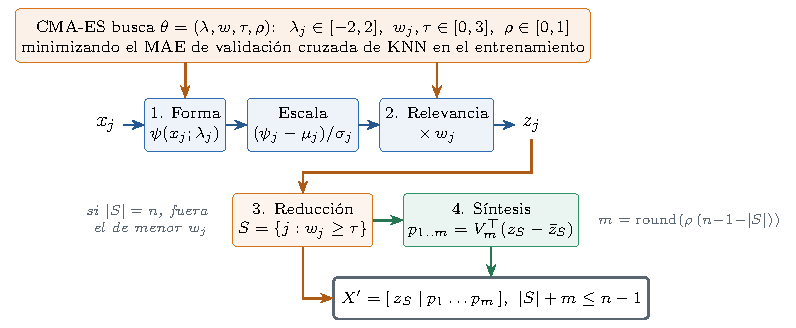
\includegraphics[width=\linewidth]{esquema}\end{center}
\vspace{2mm}
\begin{itemize}
\item \textbf{Forma}: Yeo-Johnson, $\lambda_j\in[-2,2]$. \textbf{Relevancia}: $w_j\in[0,3]$.
\item \textbf{Reducción}: fuera los atributos con $w_j<\tau$; \textbf{el umbral $\tau$ lo aprende CMA-ES}. Si no cae
ninguno, fuera el de menor peso: $\dim X'<n$ para \emph{todo} individuo, sin reparar.
\item \textbf{Síntesis}: el hueco hasta $n-1$ se rellena en una fracción $\rho$ (aprendida) con componentes
principales del espacio aprendido.
\item \textbf{CMA-ES} sobre $\theta=(\lambda,w,\tau,\rho)$, 1000 evaluaciones, fitness = MAE de VC de KNN; inicio en
la estandarización, $\sigma_0=0{,}2$.
\end{itemize}
\innerblock{Por qué reducir y sintetizar compiten}{
Añadir \emph{todas} las componentes no cambia KNN ni la R.\ lineal y da cortes oblicuos a los árboles, pero duplica
la dimensión. Con $\dim X'<n$, la síntesis compite por el hueco con los atributos originales.}
}

\block{Protocolo}{
\begin{itemize}
\item 12 datasets (diabetes, california + 10 de OpenML). Particiones 70/30 \textbf{nuevas}, no usadas para diseñar.
\item \textbf{Modelos triviales y fijos}: R. lineal, KNN ($k=5$), árbol, RF; sin ajustar. El enunciado fija $M$.
\item \textbf{Estadística por dataset} ($n=12$): Wilcoxon + Holm; Friedman + Nemenyi.
\end{itemize}
}

\block{Contraste por dataset}{
\begin{center}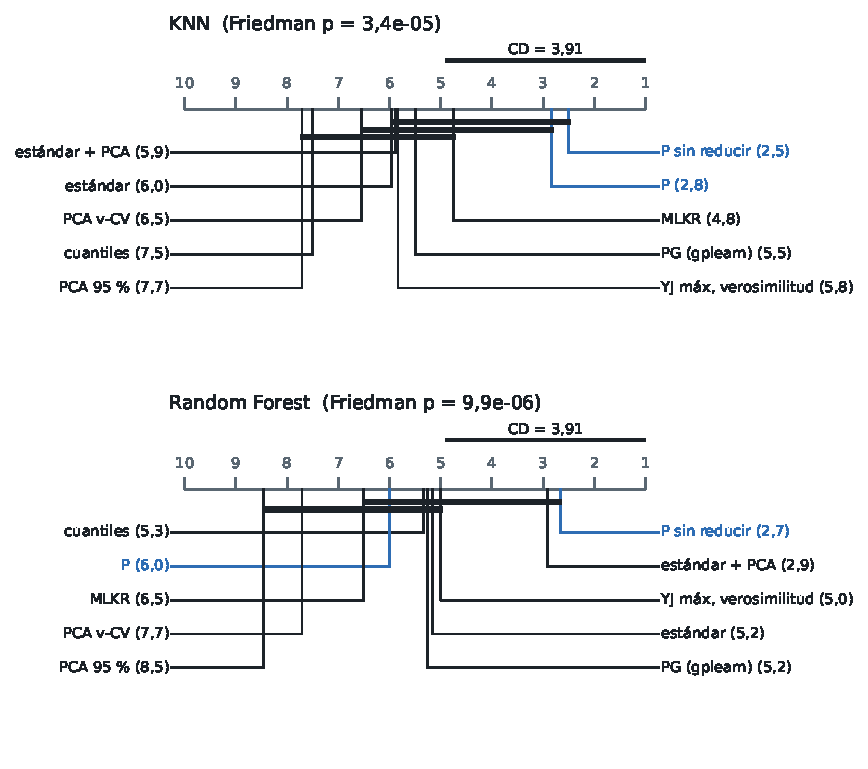
\includegraphics[width=0.8\linewidth]{poster_cd}\end{center}
{\small Nemenyi ($\alpha=0{,}05$): las barras unen transformaciones no distinguibles.}
}

% ===================================================================== columna 2
\column{0.34}
\block{3. Resultado: menos atributos, menos error en KNN y R. lineal}{
\cifra{azulm}{\dimMedia}{atributos usados de media \textbullet\ siempre $<n$}\hfill
\cifra{azulm}{\cambioKNN}{KNN \textbullet\ \dsKNN{} datasets \textbullet\ $p$=\pKNN}\\[8mm]
\cifra{azulm}{\cambioRL}{R. lineal \textbullet\ \dsRL{} datasets \textbullet\ $p$=\pRL}\hfill
\cifra{grism}{\cambioRF}{Random Forest \textbullet\ árbol \cambioArbol}
\vspace{6mm}

{\small $p$: Wilcoxon por dataset con Holm. \textbf{Concluyente en KNN}; en R.\ lineal la mejora no es
significativa con 12 datasets; en los árboles el error queda igual.}
\vspace{2mm}
\begin{center}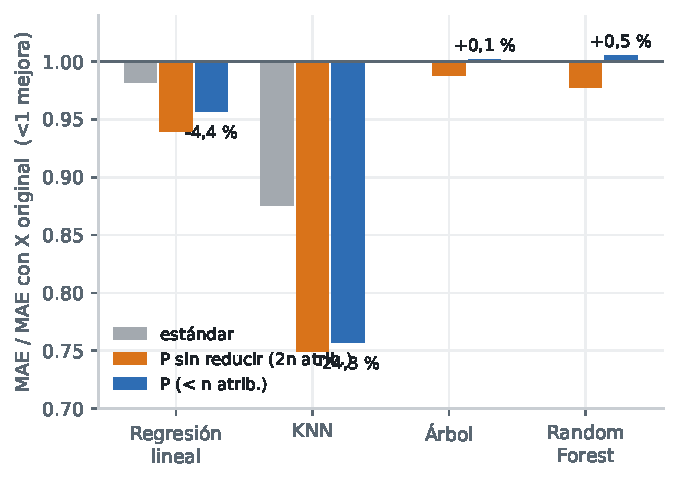
\includegraphics[width=0.95\linewidth]{poster_barras}\end{center}
\begin{center}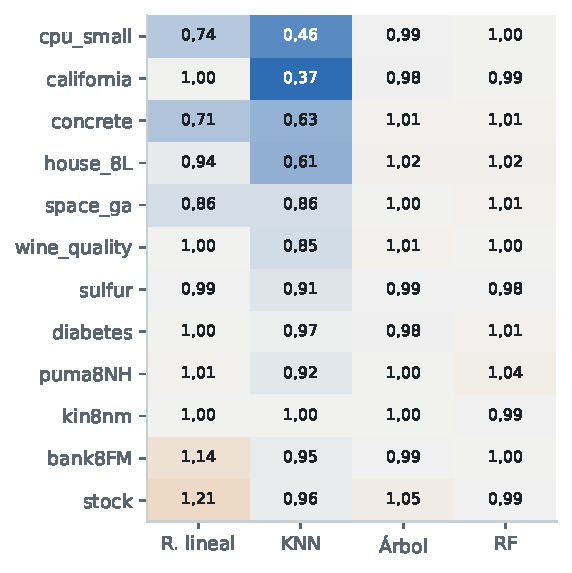
\includegraphics[width=0.85\linewidth]{poster_heatmap}\end{center}
}

\block{4. Frente a otras diez transformaciones}{
\begin{center}\small
\begin{tabular}{@{}lcccccc@{}}\toprule
 & R.\,lin. & KNN & Árbol & RF & Rango & $d/n$\\\midrule
\filasComparativa\bottomrule
\end{tabular}\end{center}
{\small $e'/e$; negrita: mejor; $^*$: $P$ mejor con $p<0{,}05$. Rango: Friedman, 1 = mejor. $d/n$: $\dim X'/n$.}
\vspace{3mm}

\textbf{Entre las transformaciones que no aumentan la dimensión, $P$ tiene el mejor rango} (\rangoP) y es la única
que reduce sin dañar a los árboles. Las tres por delante usan $2n$ atributos ($P$ sin reducir, estándar + PCA, PG).
}

\block{Coste}{
Búsqueda: \segMediana\,s de mediana por partición (1000 evaluaciones), una vez por dataset. MLKR \segMLKR\,s, PG
\segPG\,s, Yeo-Johnson MV \segYJMV\,s. Aplicarla después es inmediato, y $X'$ tiene menos columnas.
}

% ===================================================================== columna 3
\column{0.33}
\block{5. Reducción y síntesis}{
\begin{itemize}
\item CMA-ES elimina el \fracEliminados{} de los atributos ($\tau$ mediano \tauMediana); en puma8NH se queda con 2 y
añade componentes.
\item \textbf{Reducir cuesta poco}: frente a $P$ sin reducir ($2n$), KNN \cambioRedKNN, R.\ lineal \cambioRedRL; solo
RF empeora de forma significativa (\cambioRedRF).
\item \textbf{Umbral fijo} $w_j<0{,}1$: no reduce en \cribFijoNoReduce{} particiones. Aprenderlo garantiza $s<n$.
\end{itemize}
\begin{center}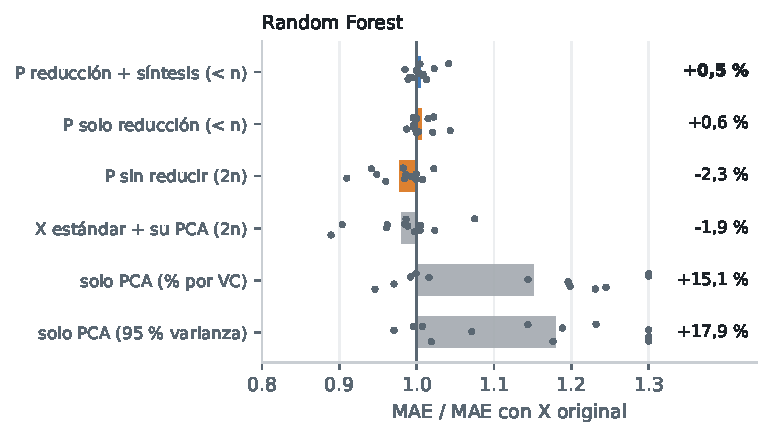
\includegraphics[width=\linewidth]{sintesis_rf}\end{center}
{\small A RF le ayuda \emph{añadir} direcciones oblicuas ($2n$); sustituir los ejes (solo PCA) lo empeora. Con
$\dim X'<n$, CMA-ES solo sintetiza en el \fracConSintesis{} de las particiones.}
}

\block{6. La búsqueda}{
\begin{center}\small
\begin{tabular}{@{}lccc@{}}\toprule
Cambio frente a $P$ & KNN & R.\,lin. & RF\\\midrule
\filasAblacion\bottomrule
\end{tabular}\end{center}
{\small $>0$: peor que $P$; $^*$: $p<0{,}05$ por dataset (Holm).}
\vspace{2mm}
\begin{itemize}
\item \textbf{Los pesos son la pieza clave}; la búsqueda gana al azar (\ctrlAleat) y a la información mutua (\ctrlMI).
\item \textbf{Población inicial}: CMA-ES es robusto; $m_0=\theta_0$ (estandarizar) se elige por interpretable.
\item \textbf{Rango} de $\lambda$: poco crítico; $[-2,2]$ evita el colapso de los $\lambda$ extremos.
\item \textbf{Algoritmo}: CMA-ES mejor en fitness (rango \rangoCMA), pero AG, HS y BBO a 1--2 puntos.
\end{itemize}
\innerblock{Operadores evolutivos}{\small
Selección por rango de $\mu=\lambda/2$ ($\lambda=$\popMin--\popMax) \textbullet\ recombinación intermedia ponderada
\textbullet\ mutación $\mathcal N(m,\sigma^2C)$ adaptativa \textbullet\ reemplazo $(\mu/\mu_w,\lambda)$ + mejor
guardado \textbullet\ parada: 1000 evaluaciones (\genMin--\genMax{} generaciones).}
}

\block{7. Conclusiones}{
\begin{itemize}
\item \textbf{$\dim X'<n$ siempre}, con el criterio de eliminación aprendido por CMA-ES.
\item $e'<e$ en KNN (\textbf{concluyente}) y R.\ lineal; árboles sin cambio.
\item \textbf{Reducir y sintetizar compiten}: a los árboles les ayuda añadir dimensiones.
\item Mejor rango entre las transformaciones que no aumentan la dimensión.
\item \textbf{La representación pesa más que el optimizador.}
\item Límites: 12 datasets pequeños; sobreajuste con pocos datos (diabetes); fitness de KNN.
\end{itemize}
}
\end{columns}
\end{document}
